%!TEX root = inversion.tex
%%%%%%%%%%%%%%%%%%%%%%%%%%%%%%%%%%%%%%%%%%%%%%%%%%%%%%%%%%%%%%%%%%%%%%%%%%%%%%
% Copyright (c) 2003-2014 by University of Queensland
% http://www.uq.edu.au
%
% Primary Business: Queensland, Australia
% Licensed under the Open Software License version 3.0
% http://www.opensource.org/licenses/osl-3.0.php
%
% Development until 2012 by Earth Systems Science Computational Center (ESSCC)
% Development 2012-2013 by School of Earth Sciences
% Development from 2014 by Centre for Geoscience Computing (GeoComp)
%
%%%%%%%%%%%%%%%%%%%%%%%%%%%%%%%%%%%%%%%%%%%%%%%%%%%%%%%%%%%%%%%%%%%%%%%%%%%%%%

\chapter{DC Resistivity Forward modelling}\label{Chp:cook:Dc Resistivity inversion}
\section{Introduction}
Dc resistivity involves placing electrodes into the ground and injecting a current
into them. The current propagates through the ground and generates a potential field.
The change in potential between a set of electrodes can then be measured. There are
a number of different ways to set up dc resistivity survey these can be found in
\cite[pg 5]{LOKE2014}. The aim of the different survey set-ups is to gather more
spacial information. Some surveys include a separation multiplier n this is because
as the separation between the electrodes increases, the current has a longer 
distance to travel and will consequently travel deeper. This is not always true
as a highly conductive layer will keep the current close to the surface.
The final objective is to perform an inversion and develop a resistivity profile of the subsurface.
This profile can then be matched up to known resistivities of material and used 
to make inferences about the material contained in the subsurface.

Escript currently supports the forward modelling of dc resistivity. Forward modelling
involves performing a survey artificially by solving the pde's which describe the underlying
physics. Escript provides a number of classes for solving forward modelling problems, these are
detailed in section \ref{sec:forward DCRES}. 

\section{Example}
In this section we will look at an example forward problem. The domain consists of
a homogenous half space with a half sphere embedded see figure \ref{fig:HalfSphere}. 
In following script~\ref{code: dc1}\footnote{The script is similar to
\examplefile{dc_forward.py} within the \escript example file directory.} run a 
Schlumberger survey on this domain.

\begin{figure}
\centering
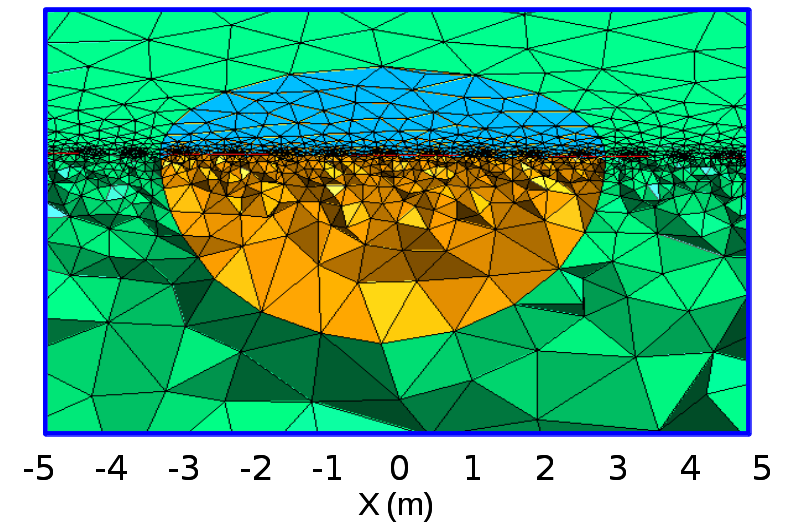
\includegraphics[width=0.7\textwidth]{HalfSphere.png}
\caption{
    (file \examplefile{data/HalfSphere_v1.4.geo}). model created using gmsh.}
\label{fig:HalfSphere}
\end{figure}

\begin{pyc}\label{code: dc1}
\
\begin{python}
#Header
import esys.finley      as finley
import esys.escript     as escript
from esys.downunder     import *
import math

#Constants
pi = math.pi

#Setup Input
mesh_file = "data/HalfSphere_v1.4.msh"
# Tag volume names and conductivity values (Sm/m) for primary and secondary potential:
tag_p = {"domain" : 1/10.0, "sphere" :  1/10.0} # Primary (homogeneous).
tag_s = {"domain" : 1/10.0, "sphere" :  1/1.0 } # Secondary.

xe_0 = -5.0 # start X-coordinate
numEle =  21  # number of electrodes
estp =  0.5 # step size
n=9 # 
midPoint = [xe_0 + (((numEle-1)*estp)/2), 0, 0]
current = 1.0 # (Ampere)
domain = finley.ReadGmsh(mesh_file, 3)
mesh_tags = escript.getTagNames(domain)
directionVector = [1,0]
sig_p = escript.Scalar(0,escript.ContinuousFunction(domain))
sig_s = escript.Scalar(0,escript.ContinuousFunction(domain))
for tag in tag_p:
    # All initially defined tags must be in the tag list.
    # Print an error if it doesn't and exit the program.
    if tag in mesh_tags:
        # Assign value:
        sig_p.setTaggedValue( tag, tag_p[tag] )
        sig_s.setTaggedValue( tag, tag_s[tag] )
    else:
        print("Error: the defined tag is not defined in the mesh: " & tag)
        sys.exit()

# Expand the data objects for output.
sig_p.expand()
sig_s.expand()
#solve for result
schs=SchlumbergerSurvey(domain, sig_p, sig_s, current, estp,n, midPoint, directionVector, nume)
pot=schs.getPotential()
totalApparentRes=schs.getApparentResistivityTotal()
#print result
n=1
print ("Total:\n")
for i in totalApparentRes:
    print ("n = %d:"%n)
    print (i,"\n")
    n=n+1
\end{python}
\end{pyc}


The example starts with by loading in a preprepared gmsh model which describes 
the domain. the gmsh script can be found in \examplefile{data/HalfSphere_v1.4.geo}
gmsh can be used to generate the msh file. The values for for primary and secondary 
conductivity is specified in the different regions. these regions have been tagged
in the gmsh script. The survey is set-up to have 21 electrodes spanning from -5 to 5
in x. Finally the potentials and total apparent resistivity is calculated. The Schlumberger
survey starts with the first 4 electrodes, with the electrode 1 and 4 as current electrodes and 
2 and 3 as potential electrodes. The electrodes used are all incremented by why before another 
measurement is taken. This is repeated until the last 4 electrodes are used. The value of n is then increased
causing the  separation between the current and potential electrodes to become 2 $\times$ a rather than a 
such that electrode 1 and 6 are current electrodes and electrodes 3 and 4 are potential electrodes. 
this process is then repeated until the maximal value of n is achieved. 
 